\documentclass[11pt]{article}
\usepackage[margin=1in]{geometry}
\usepackage{booktabs}
\usepackage{graphicx}
\usepackage{microtype}
\usepackage[hidelinks]{hyperref}

\newcommand{\NLeaves}{3,582}
\newcommand{\NAssigned}{2,918,448}
\newcommand{\LeafMedian}{349}
\newcommand{\LeafMax}{9895}


\title{\vspace{-2em}\textbf{Experiment 05 — Density-aware topic tree}}
\author{arxivkg · preprocessing · phase 5 (topic tree, offline-browse artifact)}
\date{}

\begin{document}
\maketitle
\vspace{-2em}

\section*{What we did}
Show the shape of the shipped bisecting topic tree (\texttt{leaf} + \texttt{paper\_topic}): no noise
bucket (every paper gets a leaf), the leaf-size and depth distributions, and how coherence (leaf
radius) tracks leaf size --- i.e. the coherence early-stop keeps leaves tight while adapting grain to
local density. Pure SQL + figures, no LLM; cached to \texttt{cache/summary.json}.

\section*{Summary}
\begin{center}\begin{tabular}{lr}
\toprule
metric & value \\
\midrule
leaves & 3,582 \\
papers assigned & 2,918,448 \\
leaf size min/median/p90/max & 6 / 349 / 2348 / 9895 \\
\bottomrule
\end{tabular}
\end{center}
\NLeaves{} leaves over \NAssigned{} papers (median leaf size \LeafMedian, max \LeafMax).

\begin{center}
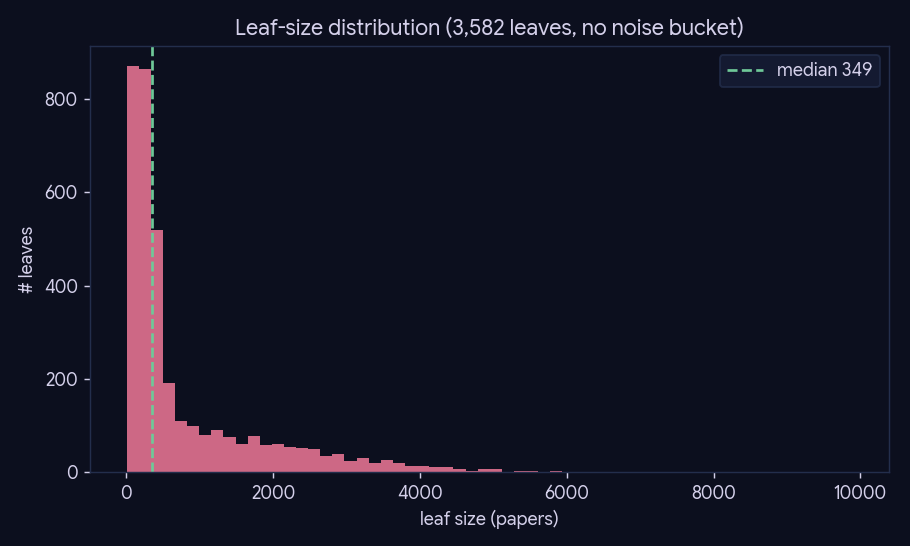
\includegraphics[width=0.6\textwidth]{../results/leaf_size.png}\\
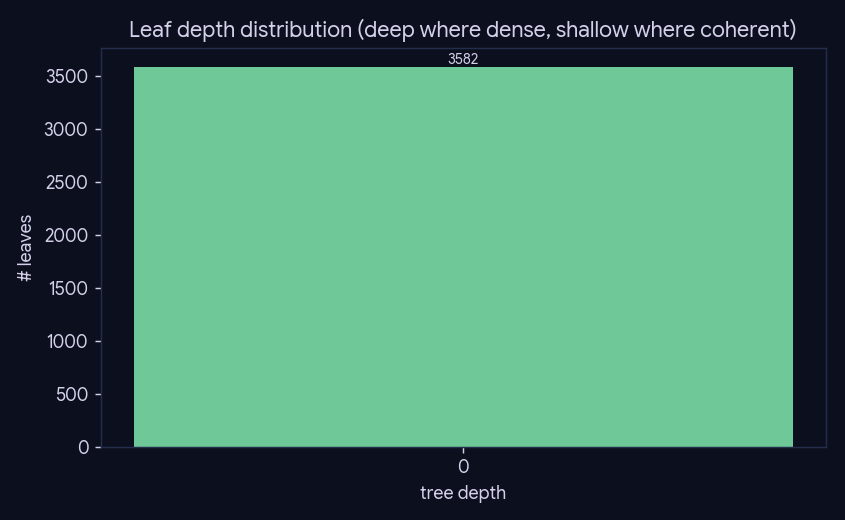
\includegraphics[width=0.55\textwidth]{../results/leaf_depth.png}
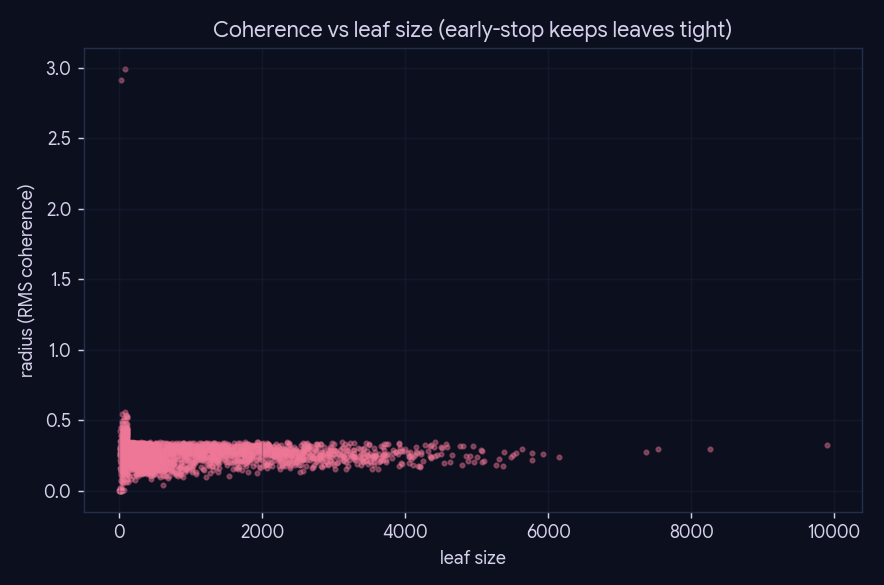
\includegraphics[width=0.55\textwidth]{../results/size_vs_radius.png}
\end{center}

\section*{Conclusion}
The tree places \textbf{all 2.92M} papers into \textbf{\NLeaves} leaves (median size \LeafMedian)
with \textbf{no noise bucket} --- the structural win over the DBSCAN-style design that dumped
$\sim$355k niche papers into a ``Miscellaneous'' sink (experiment 04). Depth is non-uniform (deeper
where dense, shallow where already coherent), and the coherence-vs-size scatter confirms the
early-stop holds leaf radius down even as leaves grow, so a topic anchor lands a query in a tight,
on-topic neighborhood. Leaf membership is from the pre-delta build (2025/2026 papers handled at serve
time by \texttt{frontier\_pull}); under the retrieval-only redesign the tree is retained only as an
offline-browse artifact.

\end{document}
